\subsection{IPTVplus and Other Pages} % (fold)
\label{sub:iptvplus}

From the main \ida{PNAI} page the user can control the sessions that are already created but, how can he create new sessions?
Another page called \idx{IPTVplus} lists all the multimedia services available to the user in categories, with thumbnails, descriptions, prices and buttons to buy that content.
Figure~\ref{fig:iptvplus} shows how the page looks.

\begin{figure}[htbp]
  \centering
    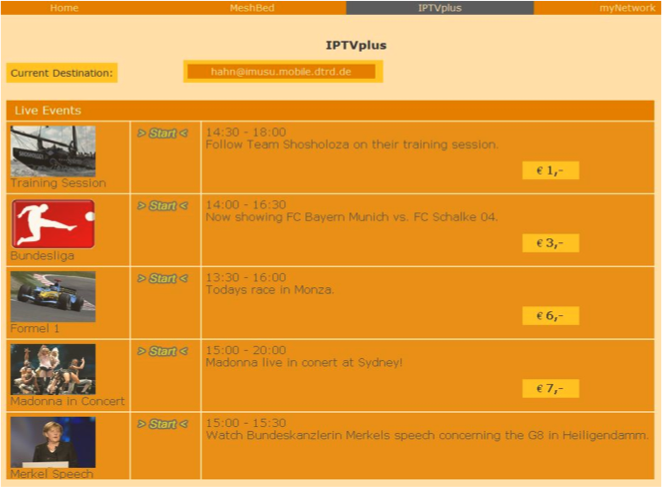
\includegraphics[width=\textwidth]{iptvplus}
  \caption{Old IPTVplus page}
  \label{fig:iptvplus}
\end{figure}

Basically, the user clicks on the button \textit{Start} to buy a content, then a popup appears to confirm the selection.
If confirmed, the user is \textit{charged} and the content starts playing in his default device.

From the user perspective this could be handled more elegantly, since the functionality is split between \idx{IPTVplus} and the \ida{PNAI}.
One of the goals of this work is integrating that functionality directly in the main \ida{PNAI} page.

This \idx{IPTVplus} application resides in a directory called \texttt{scalenet} in the \idx{Apache} public folder.
The front page from where the user accesses all the \idx{ScaleNet} applications, and therefore also the \ida{PNAI}, is in that folder.
All these pages are written in \ida{PHP}.

Figure~\ref{fig:iptvdir} lists all the relevant \ida{PHP} files in this directory.
Some folders and files have been omitted because they are not relevant to this application.

\begin{figure}[htbp]
  \dirtree{%
    .1 scalenet/.
      .2 index.php.
      .2 sub/.
        .3 includes/.
          .4 auth.inc.php.
          .4 db.inc.php.
        .3 iptvplus/.
          .4 c2d.php.
          .4 inhalt.php.
          .4 popup.php.
        .3 IPTVplus.php.
        .3 mobile/.
        .3 mobile.php.
        .3 personal/.
          .4 sessions.php.
        .3 personal.php.
  }
  \caption{Old PHP directory}
  \label{fig:iptvdir}
\end{figure}

The front page is in \idc{index.php}, and it just contains several links to the sub-applications, that are in the \idc{sub} directory.
In the \idc{includes} directory there are two files used by almost every application: \idc{auth.inc.php} for authentication purposes and \idc{db.inc.php} for connecting to the \idx{HSS DB}.

The \idc{IPTVplus.php} page is the main page for the \idx{IPTVplus} application.
This page includes \idc{inhalt.php}, where most of the actual code is written.
In short, the output of this subpage is just a list of all available videos, ordered by categories, as seen in Figure~\ref{fig:iptvplus}.

Internally \idc{inhalt.php} gets the content in a very particular way.
Instead of querying the database directly, it connects to an additional socket at \url{webportal.imusu.mobile.dtrd.de:7001} to retrieve the list.
It does not matter which component really queries the database (the \ida{SSCON}) or how, because that was not changed during this work.

To that socket it sends the string \idc{list} followed by a carriage return (\texttt{\textbackslash{}r\textbackslash{}n}).
That command responds with the information of all content items, one by one.
For each content it sends in order the following information, separated by a carriage return: \idc{type}, \idc{content}, \idc{img}, \idc{text}, \idc{lov}, \idc{priority}, \idc{price}, \idc{description} and \idc{quality}.
The end of the transmission is marked by the raw string \idc{c2d}.

The very \ida{PHP} code is rather inefficient, because it actually asks for the content four times, one for each category.
That is, it opens the socket, send the command and receive the list four times.
Each time it discards all the videos from the other categories, instead of only asking one and then ordering the results before \emph{printing} the list.

As seen in Figure~\ref{fig:iptvplus}, the list shows the title for each content (\idc{text}), its icon, its description and its price.
A button with the text \emph{Start} allows the user to buy that content, by opening a popup to \idc{c2d.php} if the content is free or to \idc{popup.php} if it is not free.

\idc{c2d.php} receives four \idc{GET} parameters: the type of the stream, the desired quality, the id of the content and the impu of the destination device/user.
The link to this \ida{PHP} file looks like this:

\texttt{.../c2d.php?type=\emph{type}\&quality=\emph{quality}\&content=\emph{content}\&}

$\hookrightarrow$\texttt{impu=\emph{destimpu}}

This script sends a command to the \ida{SSCON} to start playing that content in that device.
It opens a socket exactly like in \idc{inhalt.php} and sends the string \idc{refer} followed by the parameters separated by spaces: the destination, the \ida{SIP} id of the \idx{Application Server}, the type, the content id and the quality.
The end of the command is marked by a carriage return.

\idc{popup.php} simply contains a confirmation page asking the user if he really wants to pay for that content, and redirects the user to the \idc{c2d.php} if he confirms it.
It receives two \idc{GET} parameters: the price and the link to the proper \idc{c2d.php} page (with the needed parameters already encoded in that \idx{URL}).
The link to this \ida{PHP} file looks like this:

\texttt{.../popup.php?price=\emph{price}\&link=\emph{linktoc2d}}

\idc{mobile.php} and the files contained in the \idc{mobile} folder have a mobile version of some of this applications.
This is a very limited version and it does not contain a \idx{PNAI} page, so this files where not even touched in this work.

\idc{personal.php} is the interface that controls some things related to the user.
In the \idc{personal} folder there are several subpages that can be embedded in \idc{personal.php} depending on a \idc{GET} parameter.
One of them is \idc{sessions.php}, simply a wrapper for the \idx{PNAI} page, and it consists of an iframe redirecting to the proper path in the \ida{OSGi} server.
Therefore the \idx{PNAI} page is integrated in this portal.

There are other pages available from the same portal, some of them refers to other services (like controlling/monitoring a Mesh network) but others are configuration pages for the user.
For example, in the \idc{personal} directory there are pages to control the buddy list (add/remove), control the device list (add/remove/edit), etc.
Since those pages were left untouched by this work, they are not explained.

% subsection iptvplus (end)